\documentclass[11pt, oneside]{article} 
\usepackage[margin=1in]{geometry}  
\geometry{letterpaper}
\usepackage{graphicx}		
\usepackage{amssymb}
\usepackage[parfill]{parskip}
\usepackage{amssymb}
\usepackage{amsmath}
\usepackage{listings}
\usepackage{color}
\usepackage{standalone}
\usepackage{gensymb}
\usepackage{tikz}
\usetikzlibrary{matrix,chains,positioning,decorations.pathreplacing,arrows}
\usepackage{wrapfig}

\graphicspath{ {images/} }

\def\layersep{2.5cm}

\sloppy
\definecolor{lightgray}{gray}{0.5}
\setlength{\parindent}{0pt}
\definecolor{dkgreen}{rgb}{0,0.6,0}
\definecolor{gray}{rgb}{0.5,0.5,0.5}
\definecolor{mauve}{rgb}{0.58,0,0.82}

\lstset{frame=tb,
  language=Matlab,
  aboveskip=3mm,
  belowskip=3mm,
  showstringspaces=false,
  columns=flexible,
  basicstyle={\small\ttfamily},
  numbers=none,
  numberstyle=\tiny\color{gray},
  keywordstyle=\color{blue},
  commentstyle=\color{dkgreen},
  stringstyle=\color{mauve},
  breaklines=true,
  breakatwhitespace=true,
  tabsize=3
}

\title{Neuro 120 Homework 1: Math and Hodgkin \& Huxley}
\author{William Schmitt and Will Drew}
\date{Due: Thursday 4 October 2018 at 5pm}

\begin{document}
\maketitle

\section{Question 1: Numerical Integration}

\subsection{Implement Euler Integration}
We implement Euler Integration as follows in Matlab:
\lstinputlisting{euler_solver.m}

After changing line $29$ in \lstinline{simulate_hh.m} to \lstinline{use_euler=true}, we produce Figure \ref{fig:euler_integration_one}:

\begin{figure}[ht!]
\centering
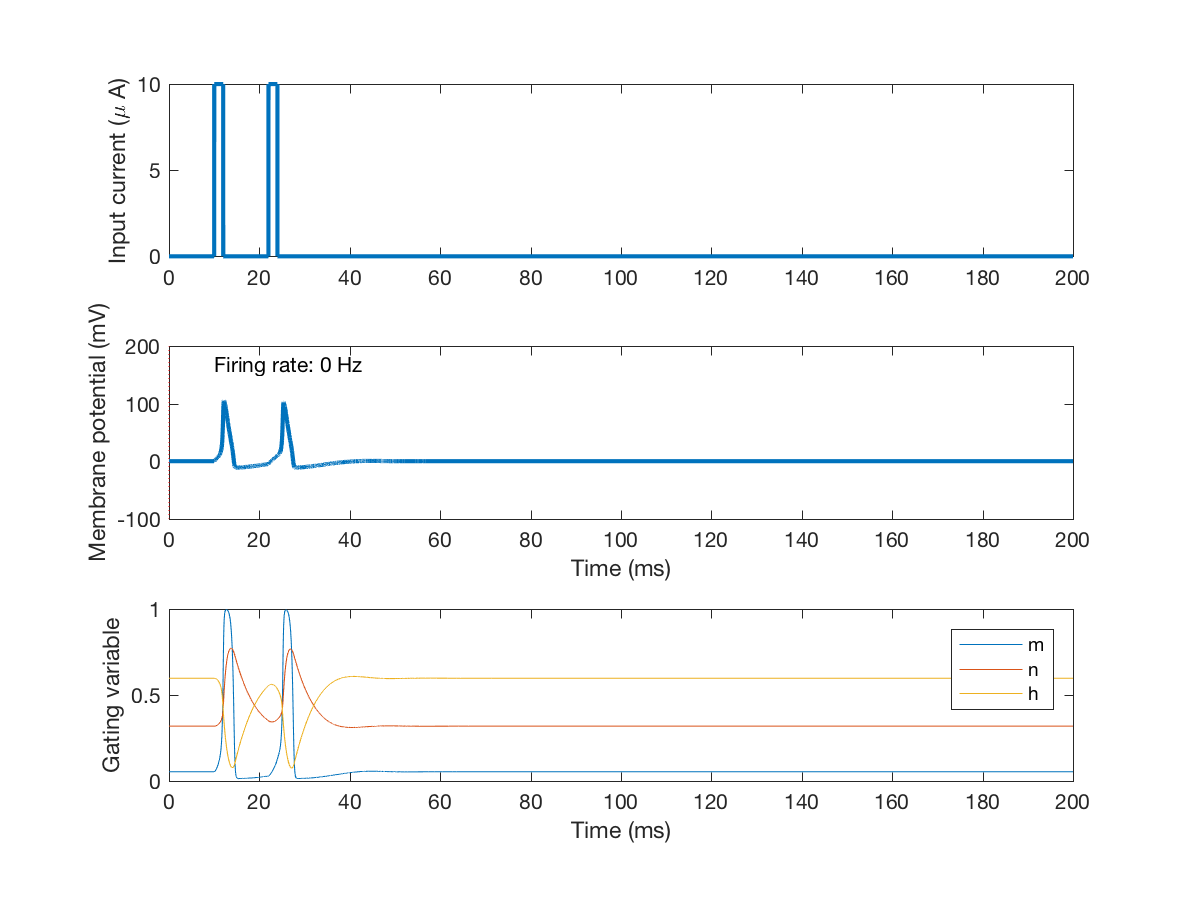
\includegraphics[width=1\textwidth]{simulate_hh_dt_1.eps}
\caption{Result of Euler Integration with $\Delta t = 0.01$.}
\label{fig:euler_integration_one}
\end{figure}

\subsection{Test Euler Integration Step Size}
We alter the setting of $\Delta t$ in \lstinline{simulate_hh.m} to $0.09$ and $0.07$ (e.g. change line 33 to \lstinline{dt = .09} or \lstinline{dt = .07}, respectively) and obtain Figures \ref{fig:euler_integration_nine} and \ref{fig:euler_integration_seven}, respectively. We see from these figures that having a step size of $0.09$ results in a failed simulation, which shows the membrane potential of the neuron going to negative infinity. This looks like it is the result of a gating variable ($m$) going to $-1$ in response to current stimulation.

\begin{figure}[ht!]
\centering
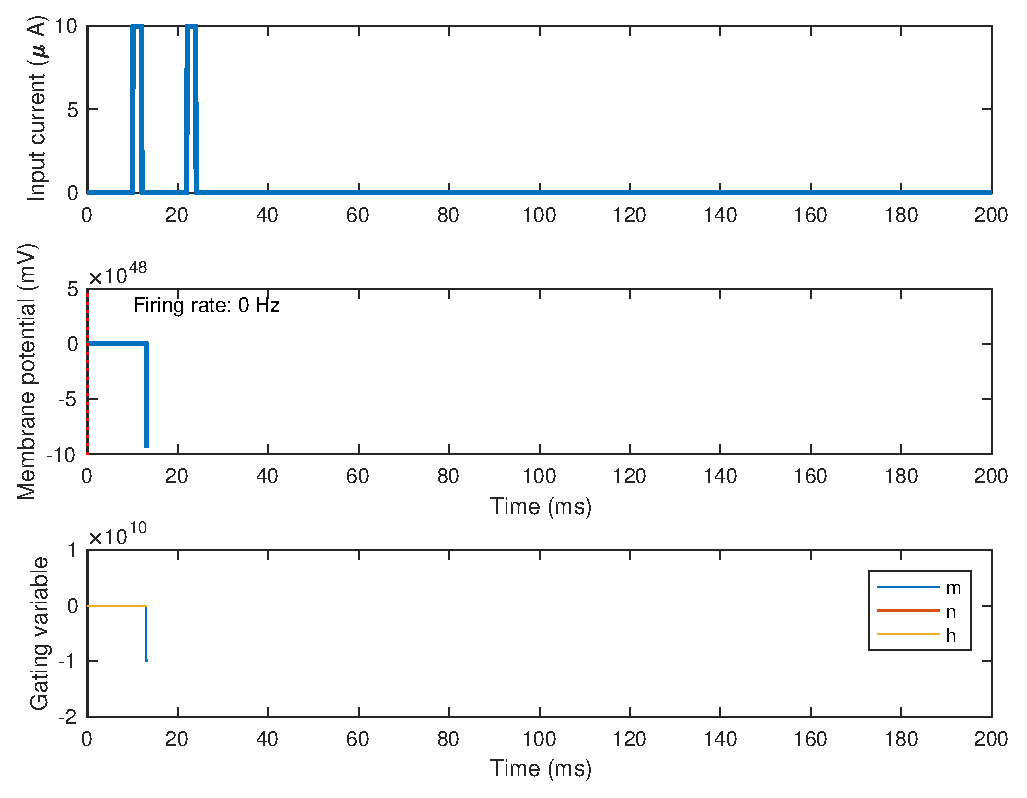
\includegraphics[width=1\textwidth]{simulate_hh_dt_9.eps}
\caption{Result of Euler Integration with $\Delta t = 0.09$.}
\label{fig:euler_integration_nine}
\end{figure}

Alternatively, when we set the step size to $0.07$, we get a simulation that looks from afar like it properly models the neural response, but upon close inspection, we can see that during the repolarization stage of the action potential, the model results in large oscillations. This indicates to us that we have too large a step size and need a smaller one in order to properly approximate the derivative of the gating variables.

\begin{figure}[ht!]
\centering
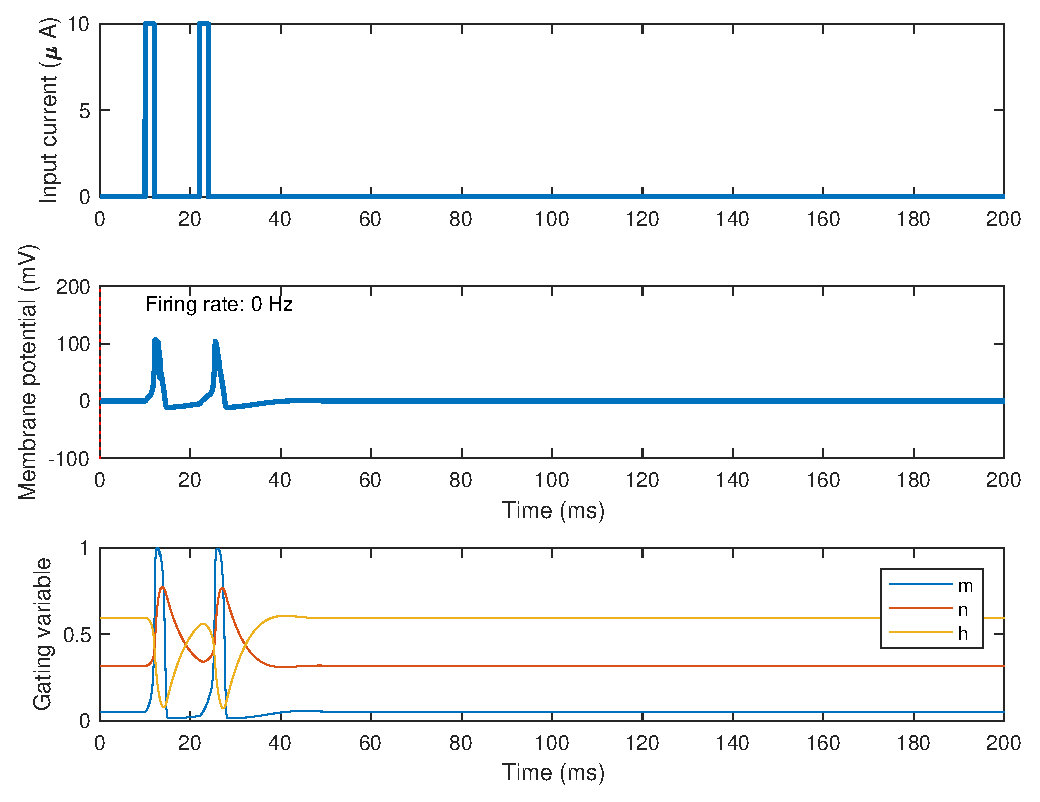
\includegraphics[width=1\textwidth]{simulate_hh_dt_7.eps}
\caption{Result of Euler Integration with $\Delta t = 0.07$.}
\label{fig:euler_integration_seven}
\end{figure}

\section{Question 2: Basic Spike Generation}
We zoom in (by using the figure tools) to the first action potential that is generated using our Euler integration model and display this in Figure \ref{fig:action_potential_close_up}. This figure illustrates how our simulated action potential slowly increases in membrane potential while there is an input current of $10\mu A$ until it hits the threshold for activation around a membrane potential of $20mV$. This activity is the result of the gating variable $m$ (which mimics the activation of a sodium channel) as we can see a similar rise in its value. After the rapid increase in the membrane potential, we see there is a rapid rise in the probability of finding a potassium channel activated (or open), which is shown by gating variable $n$. Somewhat delayed to this opening of potassium channels, the sodium channel inactivation probability increases (given by $1-h$). The combination of these two events begin to lower the membrane potential rapidly. Looking again at $m$, we see that most of the sodium channels rapidly become inactive, and now the only effect on the membrane potential is from the gating variables $n$ and $h$. These two gating variables slowly return to baseline, which results in a hyperpolarization of the membrane potential that slowly returns to baseline.

\begin{figure}[ht!]
\centering
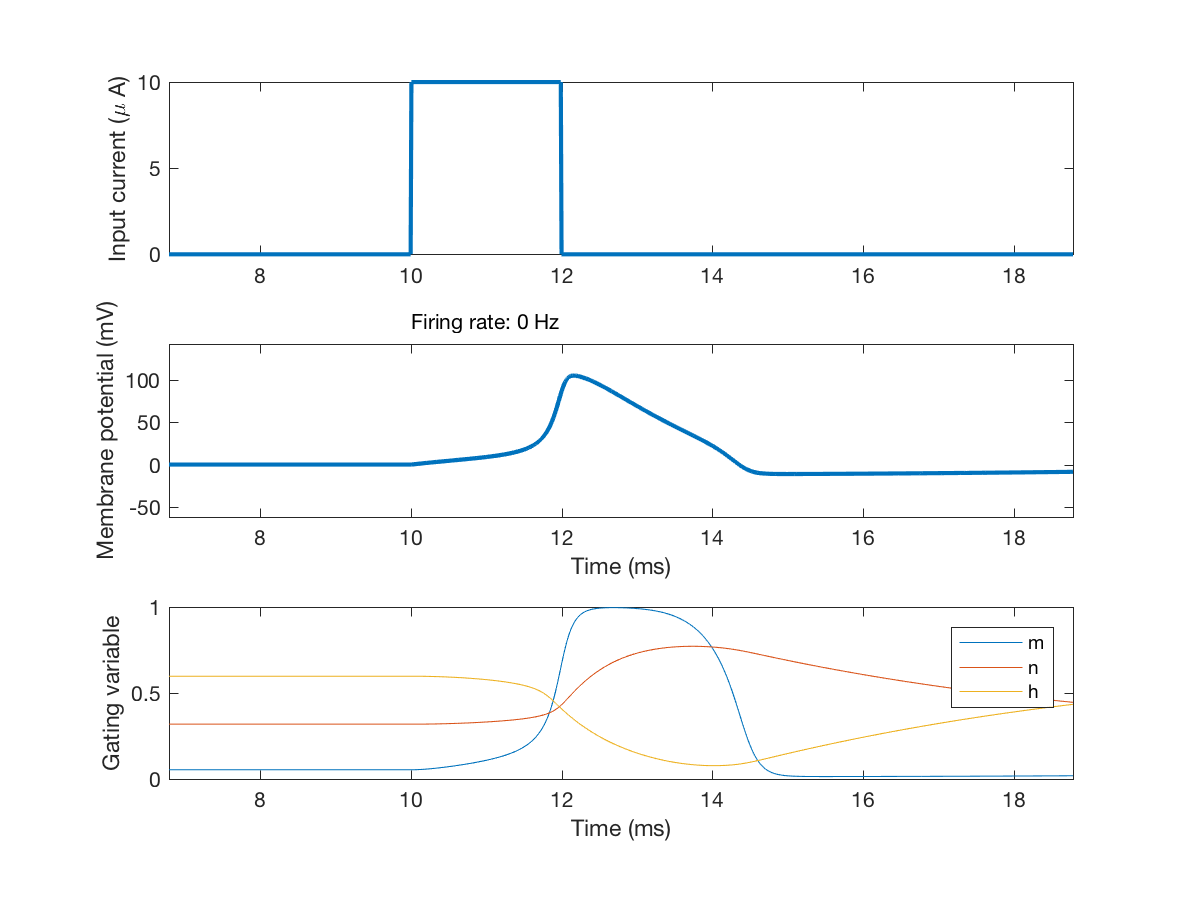
\includegraphics[width=1\textwidth]{simulate_hh_action_potential.eps}
\caption{A close-up look of a simulated action potential. Generated using the Euler integration model created in Question 1.}
\label{fig:action_potential_close_up}
\end{figure}

\section{Question 3: Firing Rate for Constant Inputs}

\subsection{The Relationship Between Firing Rate and Applied Input Current}

We created a new file called \lstinline{estimate_firing_rate.m}, which capitalizes on the code written in \lstinline{simulate_hh.m} to run a for loop to test applied input current in the range $[0, 15]$ and then plots it in Figure \ref{fig:firing_rate}. The code within this file is listed here:
\lstinputlisting{estimate_firing_rate.m}

We can see from Figure \ref{fig:firing_rate} that the simulated neuron requires at least $6 \mu A$ of applied input current in order for it to produce a sustained firing rate.

\begin{figure}[ht!]
\centering
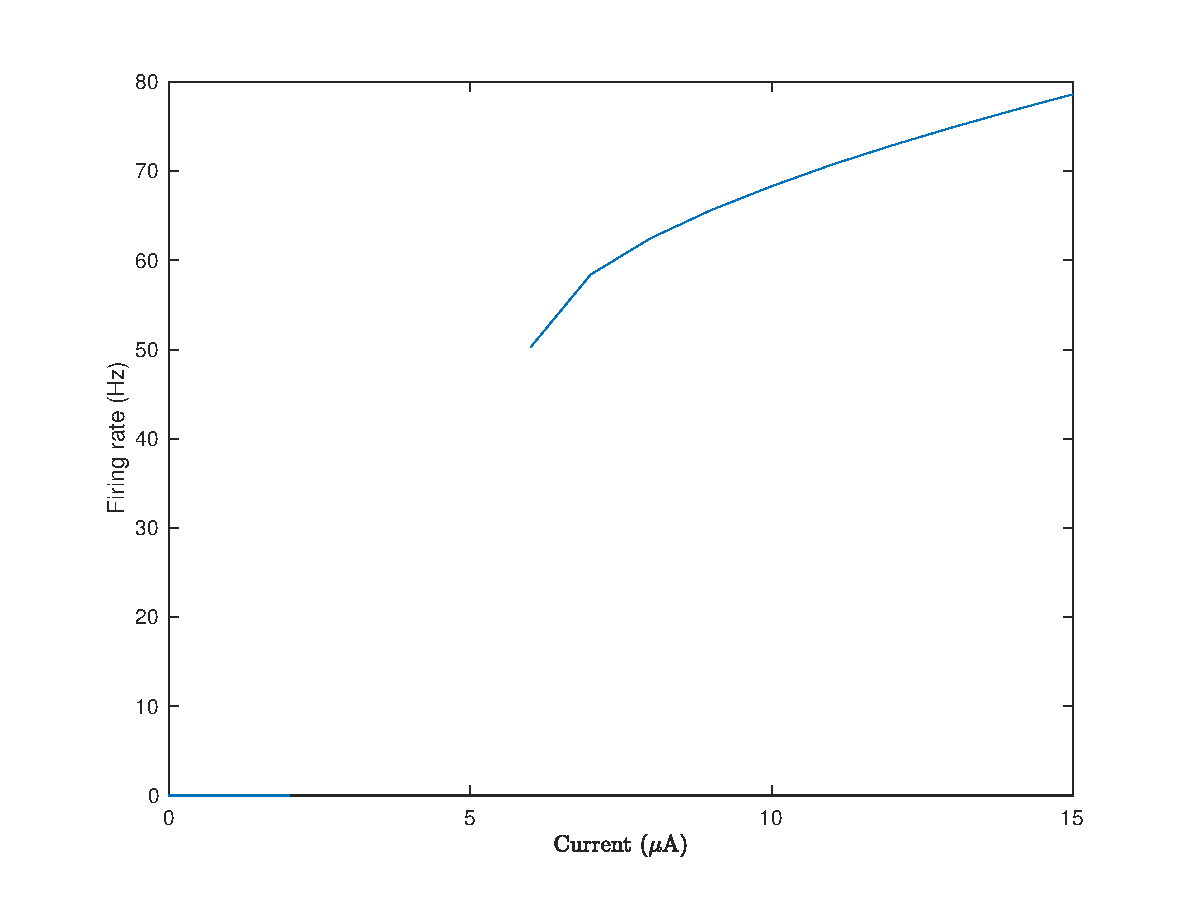
\includegraphics[width=1\textwidth]{firingrates.eps}
\caption{The firing rate of a simulated neuron as a function of the applied input current. The simulated neuron was based on a Euler integration Hodgkin-Huxley Model.}
\label{fig:firing_rate}
\end{figure}

\subsection{Minimum Sustained Firing Rate}

We can look at the vector generated by our code in \lstinline{estimate_firing_rate.m} to see that for the minimum applied current of $6\mu A$, a firing rate of 50.2260 Hz is produced. Thus, we see that the minimum sustained firing rate for this Hodgkin-Huxley model is 50.2260 Hz at this resolution ($1\mu A$) of applied input current.

\section{Question 4: Refractory Period}

\subsection{Spikes Fired for 12ms Pulse Separation}

We used a 12ms pulse separation in the applied input current in the above examples in Figures \ref{fig:euler_integration_one}-\ref{fig:action_potential_close_up}, so we can see from those results that two spikes are fired in response to these two pulses.

\subsection{Spikes Fired for 3ms Pulse Separation}

To create a 3ms pulse separation in the applied input current, we modify line 9 in \lstinline{simulate_hh.m} to be \lstinline{t_sep=3ms}. This provides the plots seen in Figure \ref{fig:3ms_separation}. We can see from this figure that two pulses separated by 3ms results in only one spike, likely due to the refractory period of this simulated neuron.

\begin{figure}[ht!]
\centering
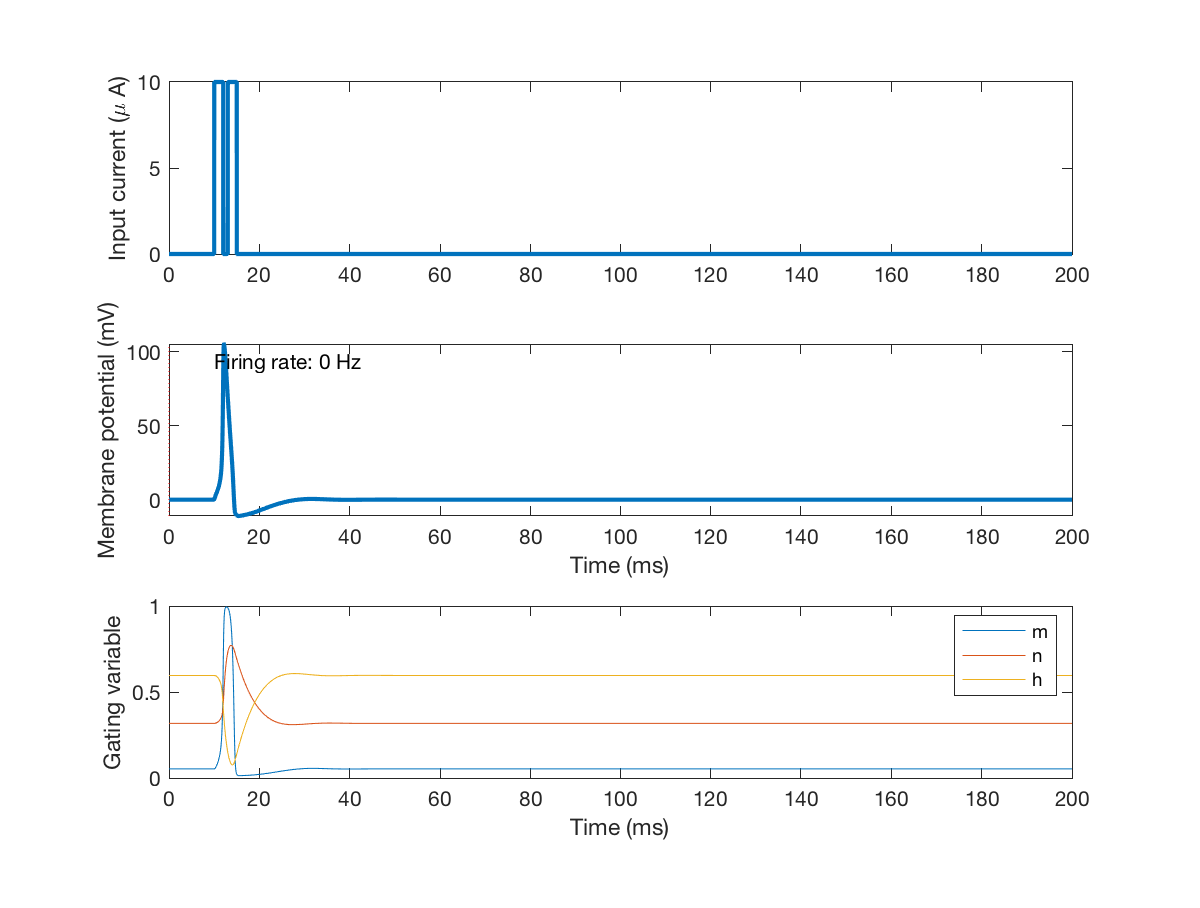
\includegraphics[width=1\textwidth]{2ms_separation.eps}
\caption{The behavior of a simulated neuron based on a Euler integration Hodgkin-Huxley Model in response to 2 3ms pulses of applied input current.}
\label{fig:3ms_separation}
\end{figure}

\subsection{Source of Refractory Period}
By looking at the gating variable behavior, we can understand why only spike was fired. When the second 3ms pulse came in, nearly all of the sodium channels were already activated (shown by gating variable $m$) and a significant portion of these were inactivated (shown by $1-h$), so the neuron could neither activate more sodium channels to increase the membrane potential nor use existing sodium channels to maintain a high membrane potential. During this time, there were also several potassium channels open, given by gating variable $n$, which would combat any possible increase in the membrane potential as this causes a decrease in the membrane potential.

\section{Question 5: History Dependence}

\subsection{Effects of Increasing Current on Firing Rate}

After uncommenting line 16 in \lstinline{simulate_hh.m}, we get Figure \ref{fig:8ma_stim}, which shows us that the firing rate of the neuron is 62.5 Hz.

\begin{figure}[ht!]
\centering
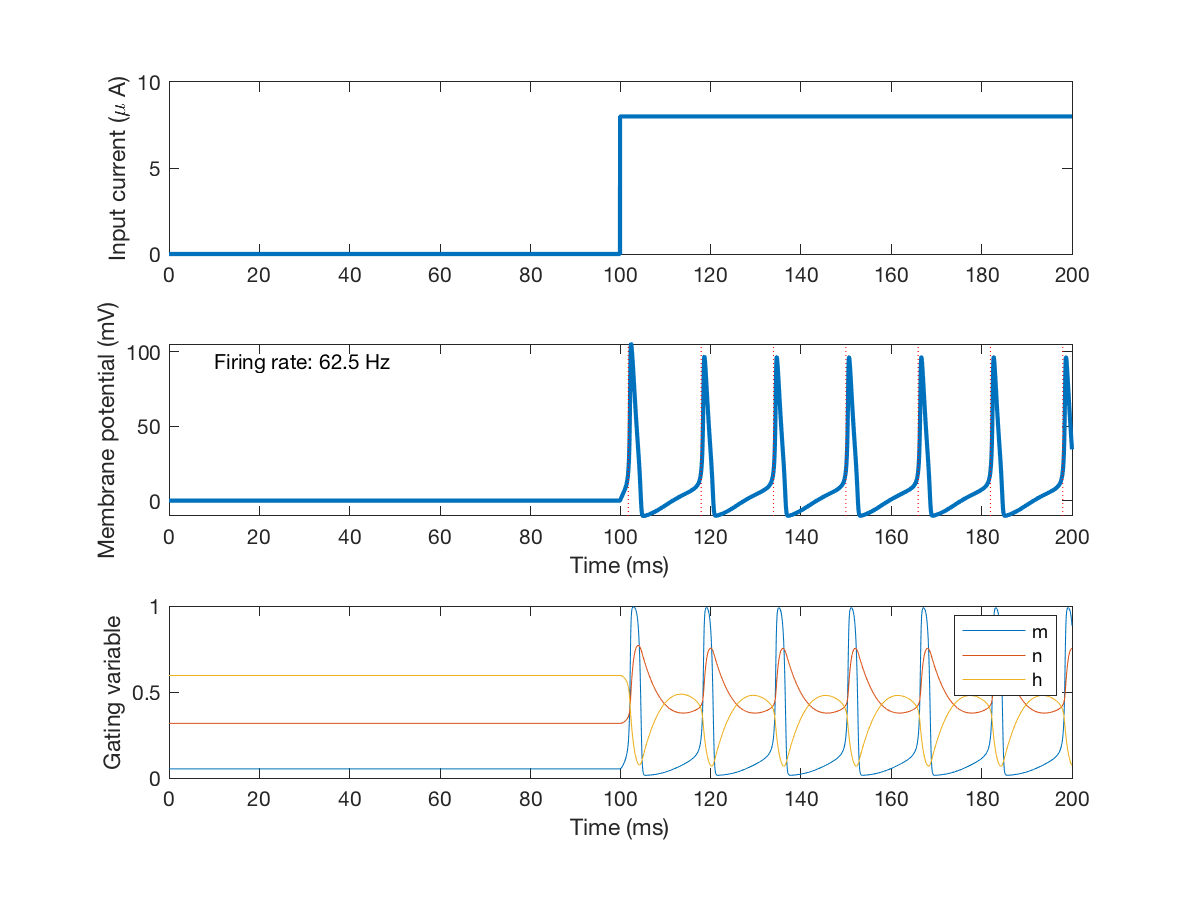
\includegraphics[width=1\textwidth]{8ma_stim.eps}
\caption{The behavior of a simulated neuron based on a Euler integration Hodgkin-Huxley Model in response to 8$\mu$A of applied input current.}
\label{fig:8ma_stim}
\end{figure}

\subsection{Effects of Decreasing Current on Firing Rate}

After uncommenting line 19 of \lstinline{simulate_hh.m}, we get Figure \ref{fig:decrease_stim}, which shows us that the firing rate of the neuron drops to 0 Hz after the drop in currrent.

\begin{figure}[ht!]
\centering
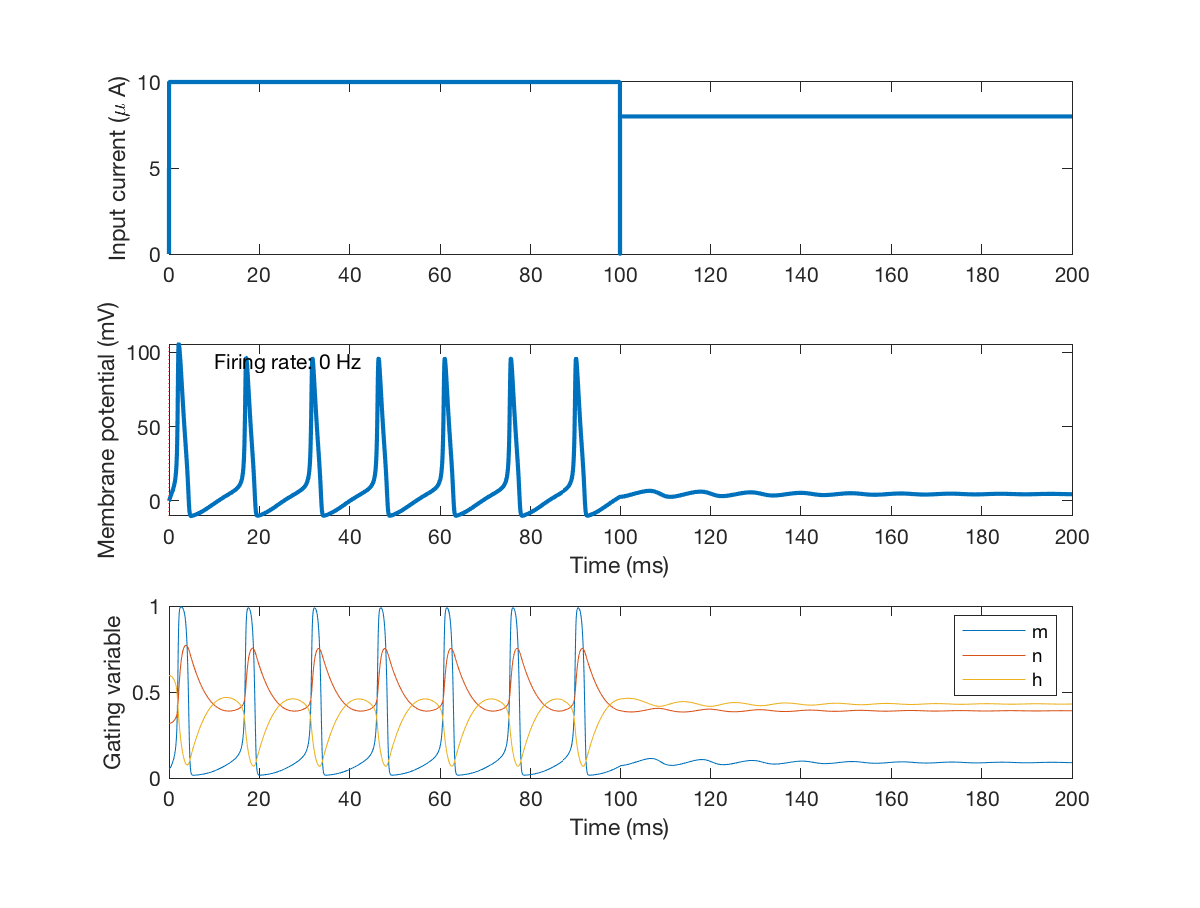
\includegraphics[width=1\textwidth]{decrease_stim.eps}
\caption{The behavior of a simulated neuron based on a Euler integration Hodgkin-Huxley Model in response to decreasing applied input current.}
\label{fig:decrease_stim}
\end{figure}

\subsection{Firing Rate Curve for $10\mu A$ to $15\mu A$}

We alter \lstinline{estimate_firing_rate.m} to test applied input currents from $10\mu A$ to $15\mu A$, and plot it in Figure \ref{fig:5c}. We see from this that it results in an increasing firing rate, which is also seen in Figure \ref{fig:firing_rate} from 3a. Checking the values of these, we see that both ranges result in the same firing rate curve.

\begin{figure}[ht!]
\centering
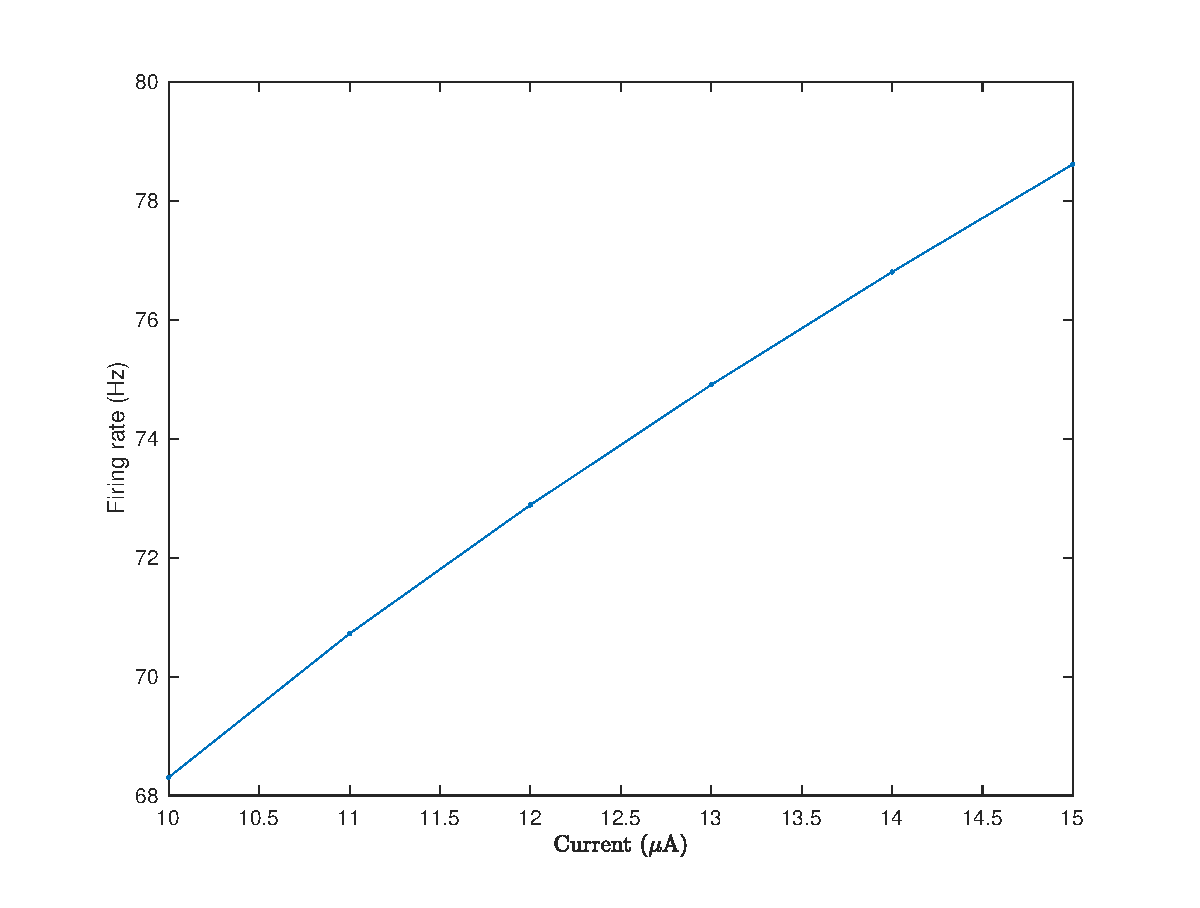
\includegraphics[width=1\textwidth]{5c.eps}
\caption{The firing rate of a simulated neuron as a function of the applied input current from $10\mu A$ to $15\mu A$. The simulated neuron was based on a Euler integration Hodgkin-Huxley Model.}
\label{fig:5c}
\end{figure}

\subsection{Effects of Turning the Current Off on Firing Rate}

We change line 19 in \lstinline{simulate_hh.m} to produce Figure \ref{fig:5d}. We see from this figure that the neuron had a steady firing rate while the current was on, and then it went back to its normal resting potential. We see from looking at the gating variables that the neuron would fire, which would place it in a refractory period (see question 4 for a description of the gating variables during this refractory period), and when the gating variables began to return to their normal state, the neuron would fire again. In particular, when the inactivation probability was low (1-h) as well as the potassium channel activation probability was low (n), the neuron would fire again. This continued until the current was turned off, at which point the gating variables returned to their baseline states.

\begin{figure}[ht!]
\centering
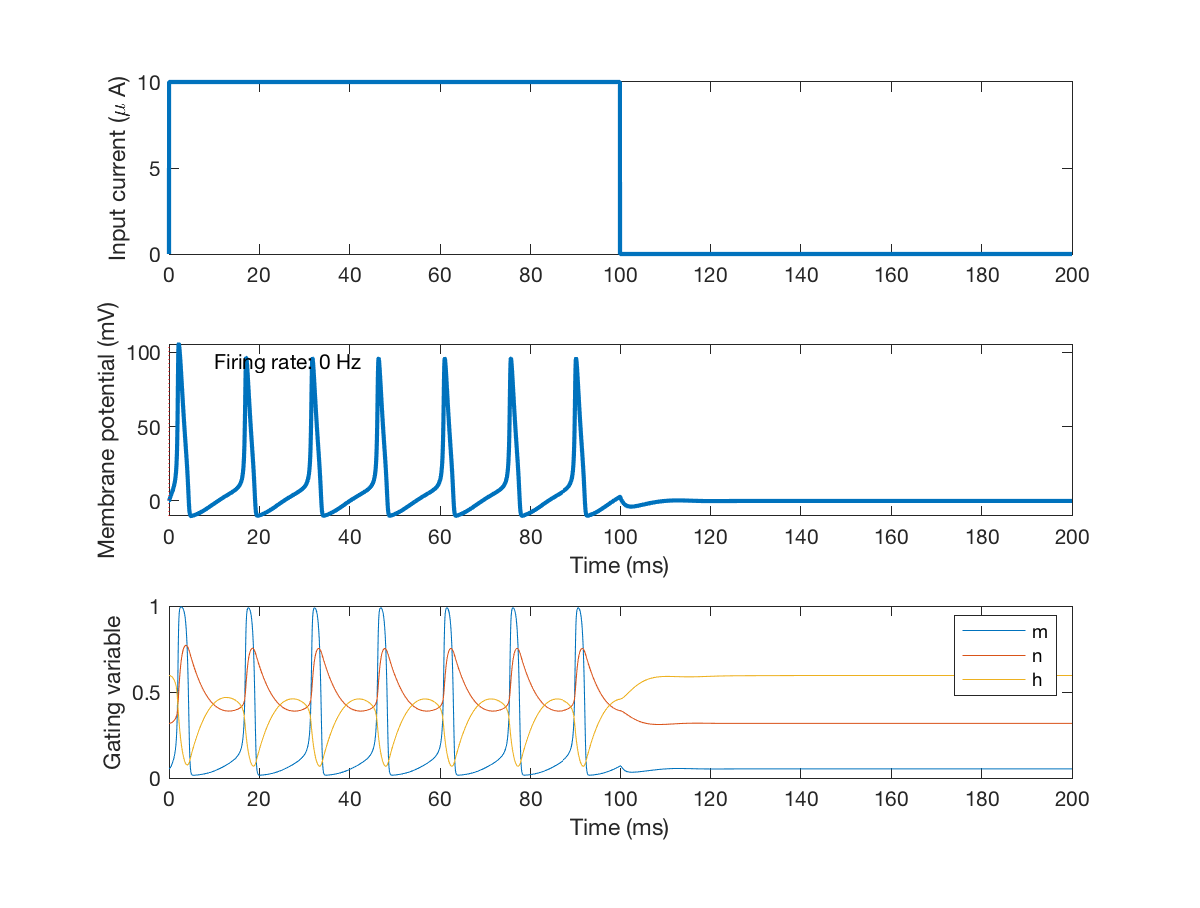
\includegraphics[width=1\textwidth]{5d.eps}
\caption{The behavior of a simulated neuron based on a Euler integration Hodgkin-Huxley Model when a $10\mu A$ applied input current is turned off.}
\label{fig:5d}
\end{figure}

\section{Question 6: Oscillations}

\subsection{Manipulation of $\omega$}

\subsection{Firing Rate Dependence on $I_0$}

\subsection{Manipulation of $I_0$}

\section{Question 7: Extra Credit: Leaky Integration}



\end{document}